%%%%%%%%%%%%%%%%%%%%%%%%%%%%%%%%%%%%%%%%%%%%%%%%%%%%%%%%%%%%%%%%%%%%%%%%%%%%%%%%
\chapter{Обзор и сравнительный анализ существующих подходов}
%%%%%%%%%%%%%%%%%%%%%%%%%%%%%%%%%%%%%%%%%%%%%%%%%%%%%%%%%%%%%%%%%%%%%%%%%%%%%%%%
В данном разделе вводятся основные определения, связанные с предметной областью, приводятся различные классификации. Рассматриваются существующие подходы к обнаружению клонов и приводятся их основные характеристики.
%%%%%%%%%%%%%%%%%%%%%%%%%%%%%%%%%%%%%%%%%%%%%%%%%%%%%%%%%%%%%%%%%%%%%%%%%%%%%%%%
\section{Основные определения и классификация}

Для рассмотрения существующих подходов к обнаружению клонов, в первую очередь необходимо дать основные определения и классификации, связанные с предметной областью. 

\begin{itemize}
\setlength\itemsep{0mm}
\item \textbf{Фрагмент кода} - часть исходного кода, необходимая для запуска программы. Такая часть может содержать в себе функцию или метод, блоки или последовательности операторов.
\item \textbf{Клон кода} - две и более части кода, которые аналогичны друг другу в соответствии с типами клонов.
\item \textbf{Клоновый класс} - максимальное множество фрагментов кода, в котором любые два фрагмента являются клонами.
\item \textbf{Кандидат в клоны} - пара фрагментов кода, которые были определены как клон.
\end{itemize}

С точки зрения идентичности дублированных фрагментов, клоны делятся на следующие типы:
\begin{itemize}
\setlength\itemsep{0mm}
\item I: Полностью идентичные фрагменты программы без учета различий разметки и комментариев \cite{surveyroyandcordy} \cite{akhinitsykson}.
\item II: Клоны идентичные клонам первого типа, в которых также не учитваются различия идентификаторов, типов и литералов \cite{surveyroyandcordy} \cite{akhinitsykson}.
\item III: Клоны, идентичные клонам второго типа, в которых также не учитываются изменения, добавления и перемешивания операторов \cite{surveyroyandcordy} \cite{akhinitsykson}.
\item VI: Фрагменты программы, решающие схожую задачу, но реализованные различными способами (семантические клоны) \cite{surveyroyandcordy} \cite{akhinitsykson}.
\end{itemize}

При рассмотрении клонов с точки зрения их размера, выделяют следующие виды:
\begin{itemize}
\setlength\itemsep{0mm}
\item С фиксированной гранулярностью: идентичные фрагменты кода фиксированного размера (методы классы и т.д.).
\item С производной гранулярностью: идентичные фрагменты произвольного размера
\end{itemize}


%%%%%%%%%%%%%%%%%%%%%%%%%%%%%%%%%%%%%%%%%%%%%%%%%%%%%%%%%%%%%%%%%%%%%%%%%%%%%%%%
\section{Причины возникновения}
%%%%%%%%%%%%%%%%%%%%%%%%%%%%%%%%%%%%%%%%%%%%%%%%%%%%%%%%%%%%%%%%%%%%%%%%%%%%%%%%

Клоны в коде не появляются сами по себе. Существует несколько причин, которые могут подтолкнуть разработчиков ко внедрению клонов в систему. Далее приведены некоторые причины их появления.

\subsection{Development strategy}

Клоны в программных системах могут появляться из-за повторного использования или programming approach. Например:

\subsubsection{Повторное использование}

Повторное использование кода, логики, дизайна и/или всей системы являются основными причинами возникновения дубликатов кода.

\textbf{Повторное использование за счет копирования/вставки}. Повторное использование кода посредством копирования/вставки (с незначительными изменениями или без них) самый простой и распространенный вид механизма повторного использования в процессе разработки. Такой способ является быстрым способом повторного использования надежных синтаксических и семантических конструкций~\cite{copypaste}.

\textbf{Ответвление}. Термин ответвление был использован Каспером и Годфри~\cite{forking} для того, чтобы обозначить повторное использование подобных решений с их возможным расхождением. Например, при разработке драйвера для семейства аппаратных устройств, похожее семейство устройств может уже иметь драйвер. Таким образом, этот драйвер может быть использован с незначительными изменениями. Аналогично, клоны могут появляться при переносе ПО с одной платформы на другую. 

\subsubsection{Programming Approach}

Клоны, также могут появляться во время разработки ПО. Например:

\textbf{Слияние двух похожих систем}. Иногда две программные системы с похожей функциональностью объединяются с целью создания новой. Также, такие системы могут быть разработаны разными командами, и, тогда, клоны при объединении появляются из-за реализации похожих функциональностей в обеих системах.

\textbf{Разработка системы с помощью генеративного подхода}. Генерация кода может породить огромное количество клонов из-за использования одинаковых шаблонов для генерации одинаковой или похожей логики.

\subsection{Maintenance benefits}

Еще одна из причин появления клонов - получение некоторых выгод обслуживания.

\textbf{Чистая и понятная архитектура ПО}. Иногда клоны намеренно внедряются в ПО для поддержания чистой и понятной архитектуры~\cite{forking}.

\textbf{Высокая стоимость вызовов функций}. В программах реального времени вызовы функций могут быть слишком затратными. В том случае, когда компилятор не предлагает встроить код автоматически, это приходится делать вручную, что непременно влечет за собой появление клонов.

\subsection{Преодоление ограничений}

Клоны могут появиться из-за различных ограничений в языках программирования.

\subsubsection{Ограничения языка}

\textbf{Significant efforts in writing reusable code}. Написание кода который потом можно будет использовать слишком трудо- и времязатратно. Поэтому, иногда проще создать клон, чем тратить силы на написание общего кода.

\textbf{Отсутствие механизма повторного использования в языке программирования}. Иногда, в языках программирования не хватает механизмов абстракции, например наследования, общих типов или передачи параметров. В следствии этого разработчикам приходится применять их как идиомы. Такие повторяющиеся действия могут создавать возможно небольшие и потенциально часто используемые клоны~\cite{javasys}~\cite{templates}.

\subsubsection{Ограничения программистов}

\textbf{Сложности в понимании больших систем}. Обычно сложно понять большую программную систему. Такие сложности толкают программистов к использованию пример-ориентированного программирования путем адаптации уже существующего кода.

\textbf{Временные ограничения}. Одними из основных причин появления клонов являются временные рамки доступные разработчикам. В большинстве случаев, разработчикам отведено ограниченное количество времени для завершения проекта или его части. Из-за таких ограничений разработчики ищут легкие пути решения проблем и, следовательно, ищут похожие существующие решения. 

\textbf{Неправильный способ измерения продуктивности}. Иногда, продуктивность разработчиков измеряется в количеством написанных строк кода в час. В таких случаях, программисты фокусируются на увеличении количества строк кода и, следовательно, пытается использовать уже существующий код.

\subsection{Случайное клонирование}

В конечном итоге, клоны могут случайно появляться в ПО.

\textbf{Протоколы взаимодействия с API и библиотеками}. Для использования API обычно требуются серии вызовов функций и/или другие последовательности команд. Например, при создании кнопки с помощью Java SWING API, серии команд включают в себя: создание кнопки, добавление ее в контейнер и назначение обработчиков событий~\cite{fingerprints}.
% \begin{figure}[htbp]
% \centering
% 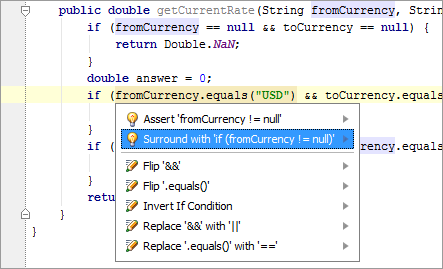
\includegraphics[width=\textwidth]{code_analysis_bugs.png}
% \caption{Рекомендации по проведению исследований в рамках диссертации}%
% \label{fig:how-to-do-research}
% \end{figure}
% 
% \Blindtext

\section{Преимущества обнаружения клонов}

Помимо очевидного понимания возможностей улучшения качества кода с помощью \textit{рефакторинга} клонов, есть и другие преимущества поиска клонов в коде. Например: 

\textbf{?Выявление кандидатов в библиотеки?}. В своих работах Дэвей~\cite{davey}, Берд и Мунро~\cite{burdmunro} отметили, что многочисленное использование скопированного кода доказывает его удобство использования. \textit{?Как результат, такой код может быть включен в библиотеку для официального объявления о своем потенциале повторного использования?}

\textbf{Помощь в понимании программы}. В том случае, когда функциональность программы осмысленна, возможно создать полную картину о других файлах, содержащих похожие копии этого фрагмента. Например, если фрагмент кода отвечает за управление памятью, можно сделать вывод, что все файлы, содержащие копию, должны иметь реализацию структуры с динамическим распределением память~\cite{memex}.

\textbf{Поиск шаблонов}. В том случае, когда все дублированные фрагменты одного исходного участка могут быть найдены, может быть обнаружена функциональная схема использования этого фрагмента~\cite{memex}.

\textbf{Поиск плагиата и нарушения авторских прав}. Поиск схожего кода может быть полезным в поиске плагиата и нарушения авторских прав~\cite{plagiat}.

\textbf{Уменьшение размера кода}. Методы поиска клонов позволяют сделать исходный код более компактным.

%%%%%%%%%%%%%%%%%%%%%%%%%%%%%%%%%%%%%%%%%%%%%%%%%%%%%%%%%%%%%%%%%%%%%%%%%%%%%%%%
\section{Критерии сравнения}
%%%%%%%%%%%%%%%%%%%%%%%%%%%%%%%%%%%%%%%%%%%%%%%%%%%%%%%%%%%%%%%%%%%%%%%%%%%%%%%%

При анализе подходов к обнаружению дублированных участков необходимо выделить основные характеристики для их сравнения. 

%%%%%%%%%%%%%%%%%%%%%%%%%%%%%%%%%%%%%%%%%%%%%%%%%%%%%%%%%%%%%%%%%%%%%%%%%%%%%%%%
\section{Способы обнаружения клонов}
%%%%%%%%%%%%%%%%%%%%%%%%%%%%%%%%%%%%%%%%%%%%%%%%%%%%%%%%%%%%%%%%%%%%%%%%%%%%%%%%

Как правило, процесс обнаружения клонов состоит из двух этапов: трансформации и сравнения. На первом этапе код преобразуется в промежуточное внутреннее представление, которое позволяет использовать более эффективные и специализированные алгоритмы сравнения. В то же время, выбор промежуточного представления накладывает ограничения на используемые алгоритмы и во многом определяет качество итоговых результатов.

Методы поиска клонов могут быть классифицированы в зависимости от способа внутреннего представления кода:
\begin{itemize}
\setlength\itemsep{0mm}
\item на основе анализа текста
\item на основе анализа токенов
\item на основе анализа синтаксических деревьев
\item на основе анализа графов
\item на основе программных метрик
\item смешанные методы
\end{itemize}

\subsection{Метод на основе анализа текста}

Подходы такого типа производят малое (или не производят вообще) количество изменений или нормализаций перед фактическим сравнением. В большинстве случаев используется непосредственно сам исходный код программы, представленный в виде последовательности строк. В полученной последовательности производится поиск одинаковых фрагментов наибольшей длины. Поиск таких фрагментов осуществляется при помощи методов анализа данных или строковых алгоритмов. К таким относятся методы сравнения отпечатков строк~\cite{fingerprints}, поиска по шаблону~\cite{templates2}, нахождения частой последовательности~\cite{sequence} и т.д.

Однако, высокая чувствительность к изменениям в исходной программе является главным недостатком подходов такого типа. Без применения модификаций такое представление позволяет обнаруживать только клоны первого типа. Для обнаружения клонов второго типа необходимо применять различного рода модификации: литералы и идентификаторы заменяются на специальные константы. Благодаря описанным модификациям, при обнаружении схожих фрагментов, такие различия не учитываются.

\subsection{Метод на основе анализа токенов}

В данном семействе подходов исходный код обрабатывается и представляется в виде последовательности, так называемых, токенов (уникальных последовательностей символов). Следующим этапом применяются строковые алгоритмы для поиска дубликатов в последовательности токенов. В отличии от методов на основе анализа текстов, такие методы позволяют использовать более эффективные и устойчивые к изменениям программы методы. Эффективность таких методов достигается за счет более компактного внутреннего представления, а их устойчивость - за счет фильтрации и нормализации токенов.

\subsection{Метод на основе анализа синтаксических деревьев}

В рамках данного подхода исходный код программы представляется в виде дерева разбора или абстрактного синтаксического дерева. Такой пожход использует структурную информацию о программе, что позволяет обнаруживать клоны первых трех типов. Однако, семантика программы не учитывается, что приводит к невозможности обнаружения клонов четвертого типа, а также клонов с измененным порядком операторов.

Для обнаружения дублированных фрагментов кода с помощью анализа деревьев, используются алгоритмы поиска одинаковых поддеревьев. Такие методы, как правило, базируются на алгоритмах динамического программирования~\cite{dynamicprog}, либо пытаются свести задачу к поиску одинаковых подстрок~\cite{substrings}. Еще оди подход, относящийся к данным рассматриваемому семейству методов - дополнение узлов дерева метриками, которые характеризуют соответствующие поддеревья	\cite{subtrees}. Такой прием сильно упрощает задачу, позволяя найти ее решение за время, пропорциональное длине исходного кода.

\subsection{Метод на основе анализа графов}



\subsection{Метод на основе программных метрик}



\subsection{Смешанные методы}


% It is of great importance that you use correct references in your dissertation.
% Resent studies show that it can increase the chances of successful defense
% by as much as 3,17 percent~\cite{russian, java-book, ANTLR}.

